% !TeX program = pdflatex
% Compilation depuis la racine : latexmk carton_invitation.tex
\documentclass[11pt,a4paper]{article}

% Encodage, langue et typographie
\usepackage[utf8]{inputenc}
\usepackage[T1]{fontenc}
\usepackage[french]{babel}
\usepackage{lmodern}
\usepackage{microtype}

% Mise en page et éléments graphiques
\usepackage[margin=22mm]{geometry}
\usepackage{graphicx}
\usepackage{xcolor}
\usepackage{tikz}
\usepackage{hyperref}
\graphicspath{{images/}}

\definecolor{BleuENS}{HTML}{007D8A}
\definecolor{Bordeaux}{HTML}{790044}
\definecolor{Encre}{HTML}{20323B}
\definecolor{GrisTexte}{HTML}{576871}
\definecolor{FondDate}{HTML}{EAF4F5}

\hypersetup{
  colorlinks=true,
  urlcolor=Bordeaux,
  pdftitle={Présentation ENS \& FAQ prépa},
  pdfsubject={Invitation à la visioconférence du 6 novembre 2026 à 18 h},
  pdfauthor={}
}


% Le lien réel reste dans un fichier local exclu de Git.
\newcommand{\LienVisio}{https://example.com/visio}
\InputIfFileExists{visio_privee.tex}{}{}

\pagestyle{empty}
\setlength{\parindent}{0pt}

\begin{document}
\sffamily
\color{Encre}

% Les positions fixes assurent une page unique et un titre légèrement au-dessus du centre.
\begin{tikzpicture}[remember picture,overlay]
  \draw[BleuENS,line width=1.3pt]
    ([xshift=22mm,yshift=-15mm]current page.north west) --
    ([xshift=-22mm,yshift=-15mm]current page.north east);

  % Logos d'origine, conservés sans déformation.
  \node[anchor=north west,inner sep=0pt]
    at ([xshift=24mm,yshift=-23mm]current page.north west)
    {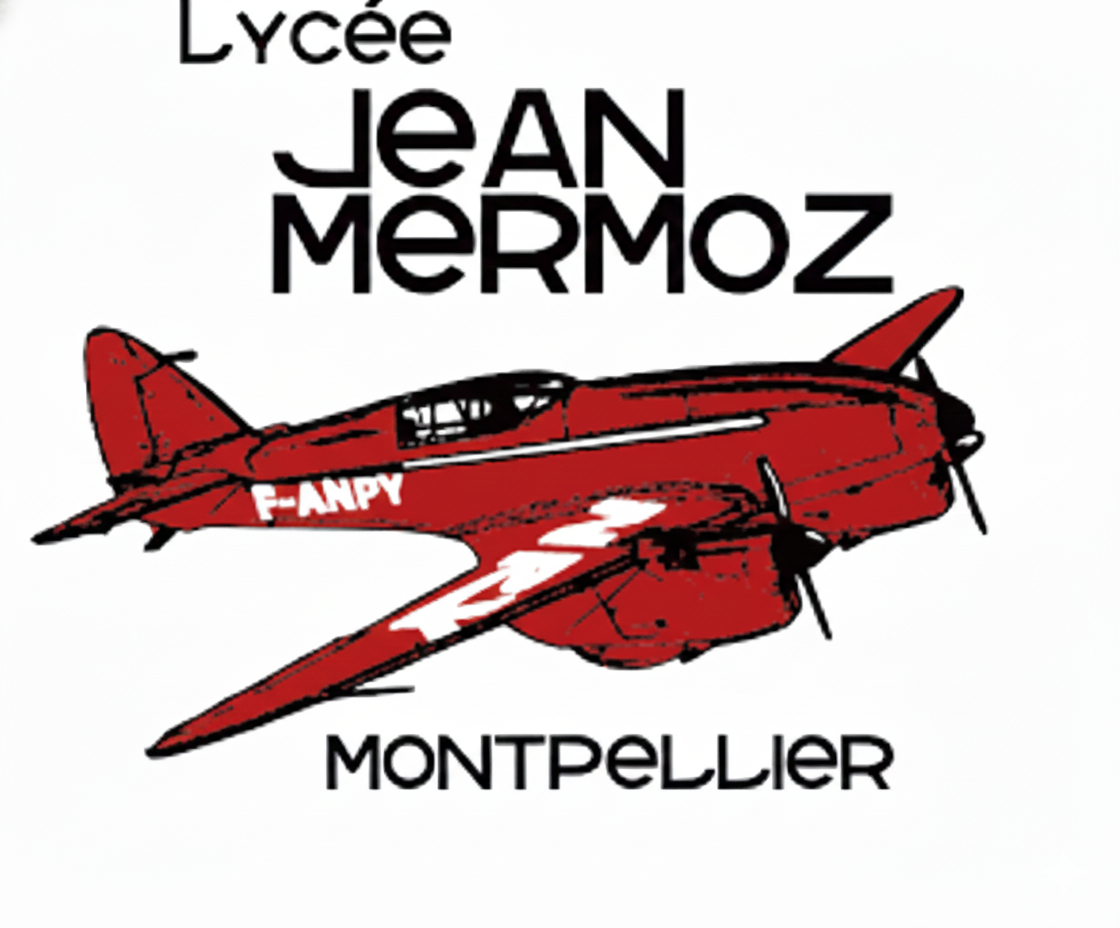
\includegraphics[width=31mm]{logo_mermoz(1).png}};
  \node[anchor=north east,inner sep=0pt]
    at ([xshift=-24mm,yshift=-28mm]current page.north east)
    {
\includegraphics[width=72mm]{logo_ens_ups(1).png}};


  % Titre centré horizontalement, 20 mm au-dessus du centre de la page.
  \node[anchor=center,inner sep=0pt,text width=166mm,align=center]
    at ([yshift=20mm]current page.center)
    {{\fontsize{30}{35}\selectfont\bfseries
       Présentation ENS\\[1mm]\& FAQ prépa\par}};

  % Date et horaire mis en évidence, sans indication de durée.
  \node[fill=FondDate,rounded corners=2mm,inner xsep=10mm,inner ysep=6mm]
    at ([yshift=-35mm]current page.center)
    {{\Large\bfseries\color{BleuENS} 6 novembre 2026}
     \hspace{6mm}{\large à}\hspace{6mm}
     {\LARGE\bfseries\color{Bordeaux} 18\,h}};

  % Toute la surface du bouton est cliquable.
  \node[inner sep=0pt] at ([yshift=-65mm]current page.center)
    {\href{\LienVisio}{%
      \setlength{\fboxsep}{0pt}%
      \colorbox{Bordeaux}{%
        \parbox[c][15mm][c]{78mm}{%
          \centering\color{white}\Large\bfseries rejoignez ici}%
      }%
    }};
  \node[inner sep=0pt,text=GrisTexte,font=\small]
    at ([yshift=-16mm]current page.center)
    {};

  % % Texte d'accompagnement.
  % \node[inner sep=0pt,text width=142mm,align=center]
  %   at ([yshift=-57mm]current page.center)
  %   {{\large\bfseries Découvrir l'ENS Paris-Saclay}\par
  %    \vspace{4mm}
  %    {\normalsize Un échange autour de l'École normale supérieure\par
  %     et de vos questions sur la prépa.}\par
  %    \vspace{7mm}
  %    {\normalsize\color{BleuENS} Vos questions sont les bienvenues !}};

   \draw[BleuENS!30,line width=0.5pt]
     ([xshift=22mm,yshift=30mm]current page.south west) --
     ([xshift=-22mm,yshift=30mm]current page.south east);
  % \node[inner sep=0pt,text=GrisTexte,font=\small]
  %   at ([yshift=23mm]current page.south)
  %   { \quad\textbullet\quad };
\end{tikzpicture}
\null
\end{document}
